\documentclass[10pt]{article}
%
\usepackage{a4wide}
\usepackage{amsmath}
\usepackage{graphics,subfig}

\usepackage{tikz}
\usepackage{pgfkeys}
%
\usetikzlibrary{shapes}
% p 48
\title{Distribution of particles into ScalFMM}
\author{O. Coulaud}
\date{March, 29th 2014\\\vspace{1cm}Version 0.1}
\begin{document}
\maketitle

\tableofcontents
\newpage
\section{Uniform distribution for surface}

For parametric surface, J  Williamson in \cite{Williamson} proposed a method to construct uniform distribution of points on such surface. For ellipsoid, this method was improved in \cite{ChenGlotzer}. Here we follow their approach to construct uniform distribution.

\subsection{Sphere distribution}
Consider that we want $N$ point uniformly set on the surface of the unit sphere, the natural choice is to sample uniformly the angles $\theta$ and $\phi$ of the spherical coordinates. Unfortunately, such choice lead to a concentration of points near the pole.  As a surface area is given by $sin\phi\,d\phi\,d\theta = -d(cos\phi)\,d\theta$, we will sample $cos\phi$ rather than $\Phi$. So, we choose $u$ and $v$ two  random variable on [0,1] and  
\begin{eqnarray*}
\theta	&=&	2\pi u,\\
\phi	&=&	cos^{-1}(2v-1).
\end{eqnarray*}
then we obtain a uniform distribution of points on the unit sphere.

\begin{figure}[ht]
  \centering
   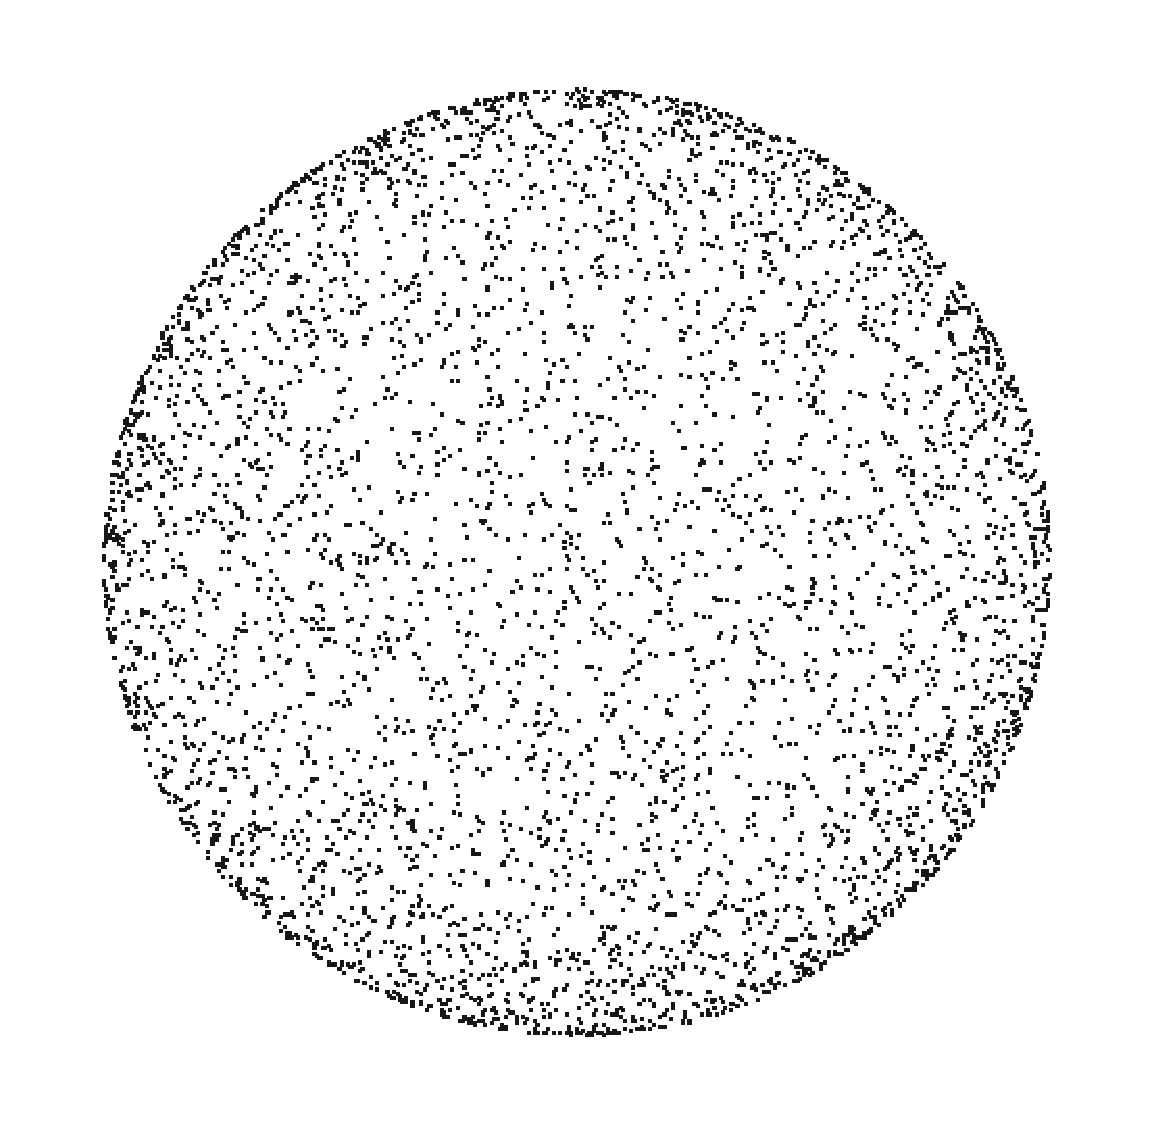
\includegraphics[width=0.3\textwidth]{unitsphere}
    \caption{$5\,000$ points distribution on unit sphere.}%
\end{figure}
\texttt{generateDistributions -unitsphere   -N 5000 -fout unitsphere.fma -fvisuout unitsphere.vtp }


\subsection{Ellipsoid distribution}
Here we want to construct a uniform distribution on an ellipsoid defined by the equation
\begin{equation}
f(x,y,z) = (\frac{x}{a})^2+(\frac{y}{b})^2+(\frac{z}{c})^2-1,
\end{equation}
and the parameterization 
\begin{eqnarray*}
x	&=&	a\cos(u)\cos(v),\\
y	&=&	b\cos(u)\sin(v), \\
z  &=&	c\sin(u).
\end{eqnarray*}
with $u\in [0, 2\pi[$ and  $v\in [0, \pi[$. if you sample $u$ and $v$ then we obtain a non uniform distribution on the ellipsoid see section~ \ref{nonuniEllipsoid}.
\subsubsection{prolate}
A prolate spherical geometry is an ellipsoid where $a=b$ and $c>a$. On the case $g_{max}=1+a^2$ is obtain when $z=o$. Then to construct a uniform distribution we proceed as follow
\begin{description}
\item[step 1] Build a uniform point on the sphere and map it on the prolate surface. Let u a random point in $[-1,1]$ and v in $[0,\pi]$, then 
\begin{eqnarray*}
x	&=&	a\sqrt{1-u^2}\cos(v),\\
y	&=&	b\sqrt{1-u^2}\sin(v), \\
z  &=&	c u.
\end{eqnarray*}
\item[step 2] Correct the distribution.  Choose a random point $\xi$ in $[0,1]$ and if 
$$ x^2+y^2 + \frac{a^4}{c^4} z^2 < a^2 \xi^2 $$
is true then we keep the point otherwise we reject it.
\end{description}
\begin{figure}[h]
  \centering
  \begin{minipage}{0.45\textwidth}%
   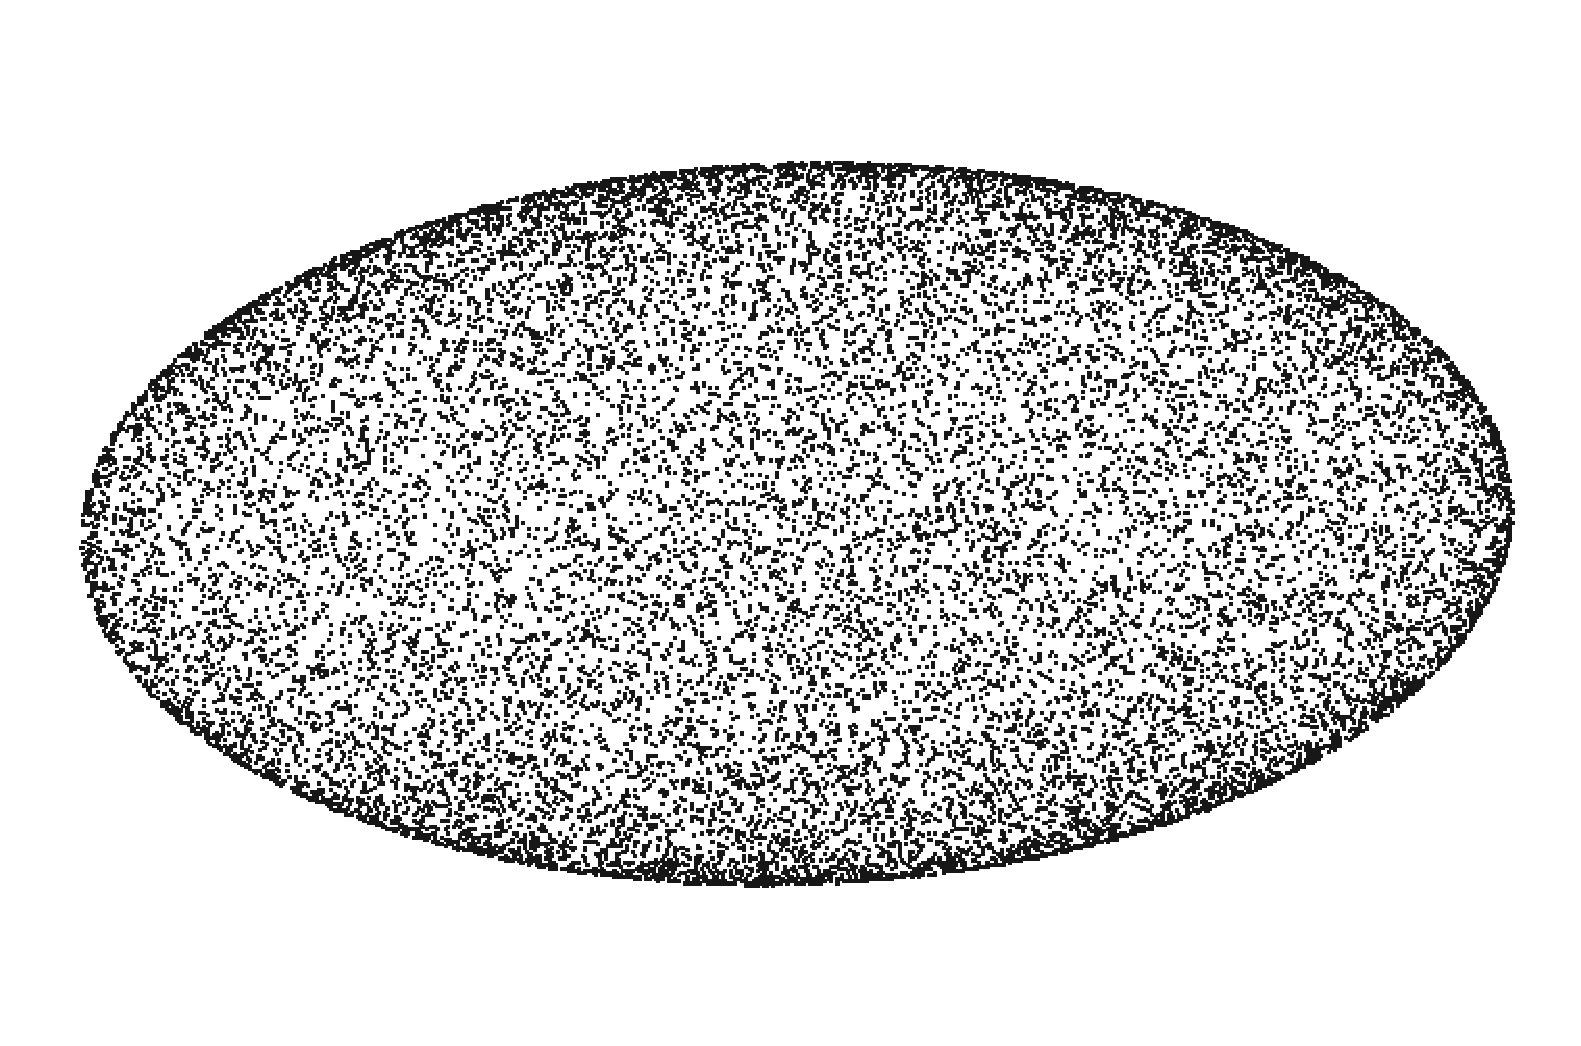
\includegraphics[width=1.0\textwidth]{ellipsoidUnif}
    \caption{$20\,000$ points distribution on 2:2:4 ellipsoid. Less than $15 \%$ of points has been rejected.}%
      \end{minipage}%
  \qquad
  \begin{minipage}{0.45\textwidth}%
   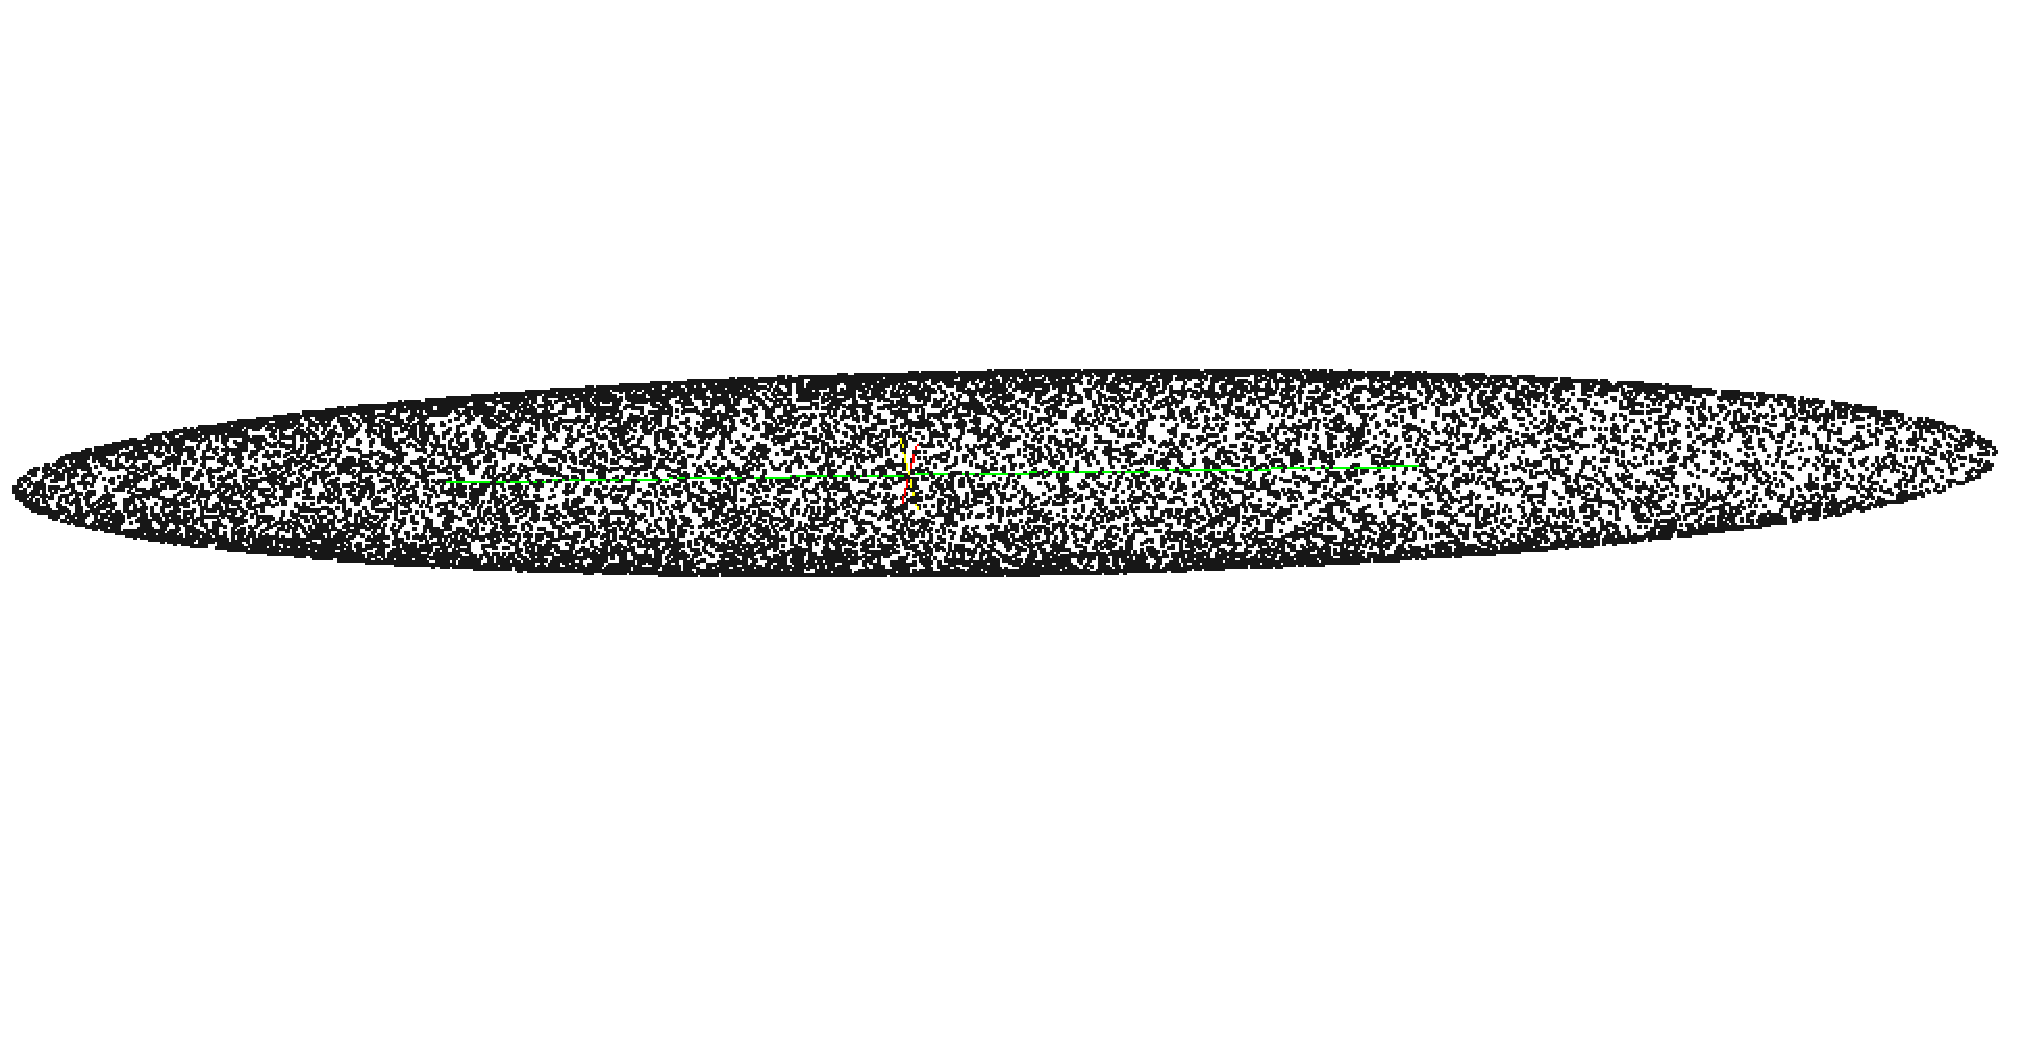
\includegraphics[width=1.2\textwidth]{prolate}
    \caption{$20\,000$ points distribution on 1:1:10 ellipsoid and only $21\%$ of the tested points in step 2 has been rejected.}%
%    \label{fig:2figsB}%
  \end{minipage}%
\end{figure}

\texttt{generateDistributions -prolate -ar 1:1:10   -N 20000 -fout prolate.bfma -fvisuout prolate.vtp}



\section{Non uniform distribution}

\subsection{Ellipsoid}
\label{nonuniEllipsoid}
The simplest way to sample and ellipsoid of size a:b:c is to consider its spherical coordinates. Let $u$ and $v$ two random numbers between 0 and 1. After mapping u (resp. v) in $[-\pi/2,\pi/2]$ resp. ($[-\pi,\pi]$), the Cartesian coordinates are    
\begin{eqnarray*}
x	&=&	a\cos(u)\cos(v),\\
y	&=&	b\cos(u)\sin(v), \\
z  &=&	c\sin(u).
\end{eqnarray*}
As shown in the figure~\ref{Fig-nonUnifEllipsoid} we obtain a concentration of points near the poles $(0,0,\pm c)$.
\begin{figure}[hbt]
  \centering
   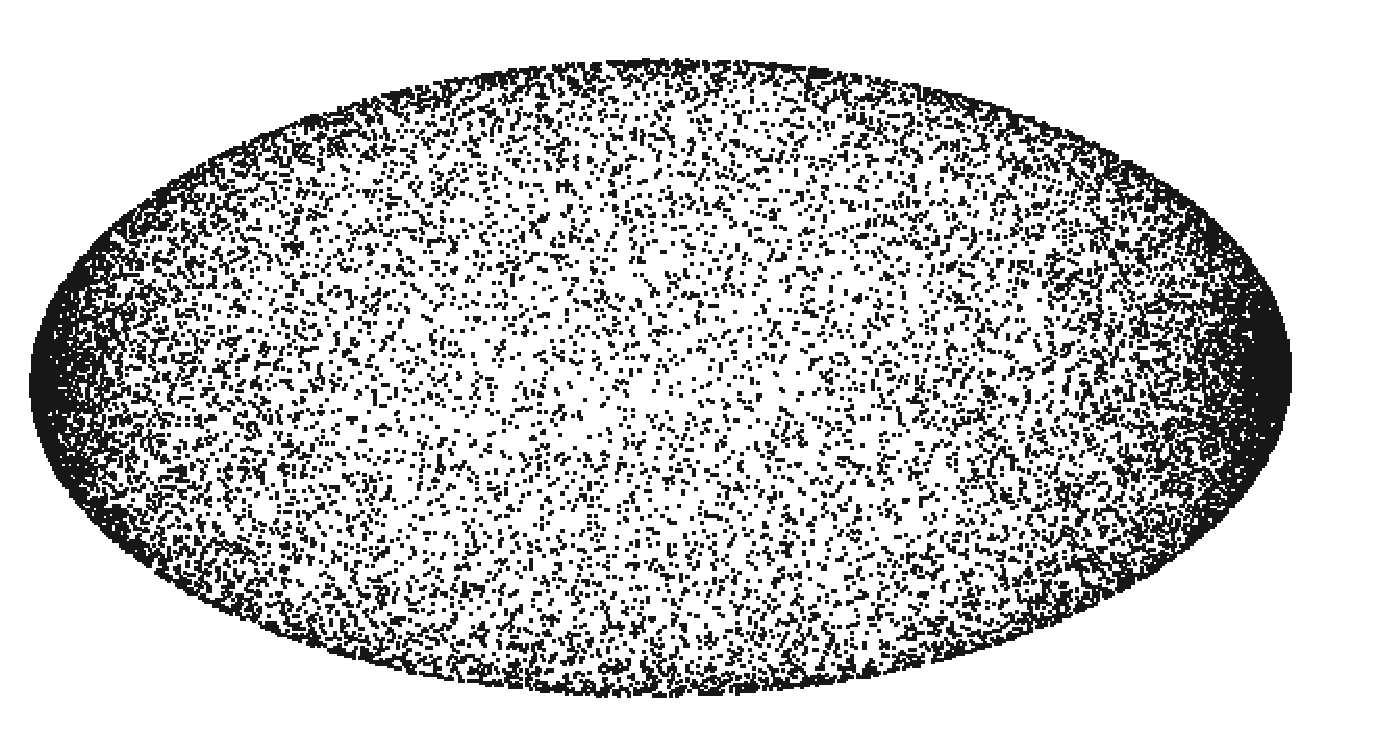
\includegraphics[width=0.5\textwidth]{ellipsoid}
    \caption{$20\,000$ points distribution on an ellipsoid of aspect ratio 2:2:4.}%
    \label{Fig-nonUnifEllipsoid}
\end{figure}
This bias on the pole could be reduced by choosing the same approach that we use to build a uniform distribution on the unit sphere?


\texttt{generateDistributions -ellipsoid -ar 2:2:4   -N 20000 -fout ellipsoid.bfma  -fvisuout ellipsoid.vtp}

If you consider the 

\subsection{Plummer Model}
This is a hard test case in astrophysics problem, and it models a globular cluster of stars, which is highly non uniform.  It is called   the plummer distribution. To construct such distribution, first we construct a uniform points distribution on the unit sphere. Second, the radius is chosen according to the plummer distribution (double power law in astrophysics). We consider $u$ a random number between 0 and 1, then the associated radius is given by
\begin{equation*}
r = 1.0/\sqrt{u^{-2/3}-1},
\end{equation*}
and the total mass is one. Then, $m_i = \frac{1}{Npt}$.
\begin{figure}[h]
  \centering
  \begin{minipage}{0.45\textwidth}%
    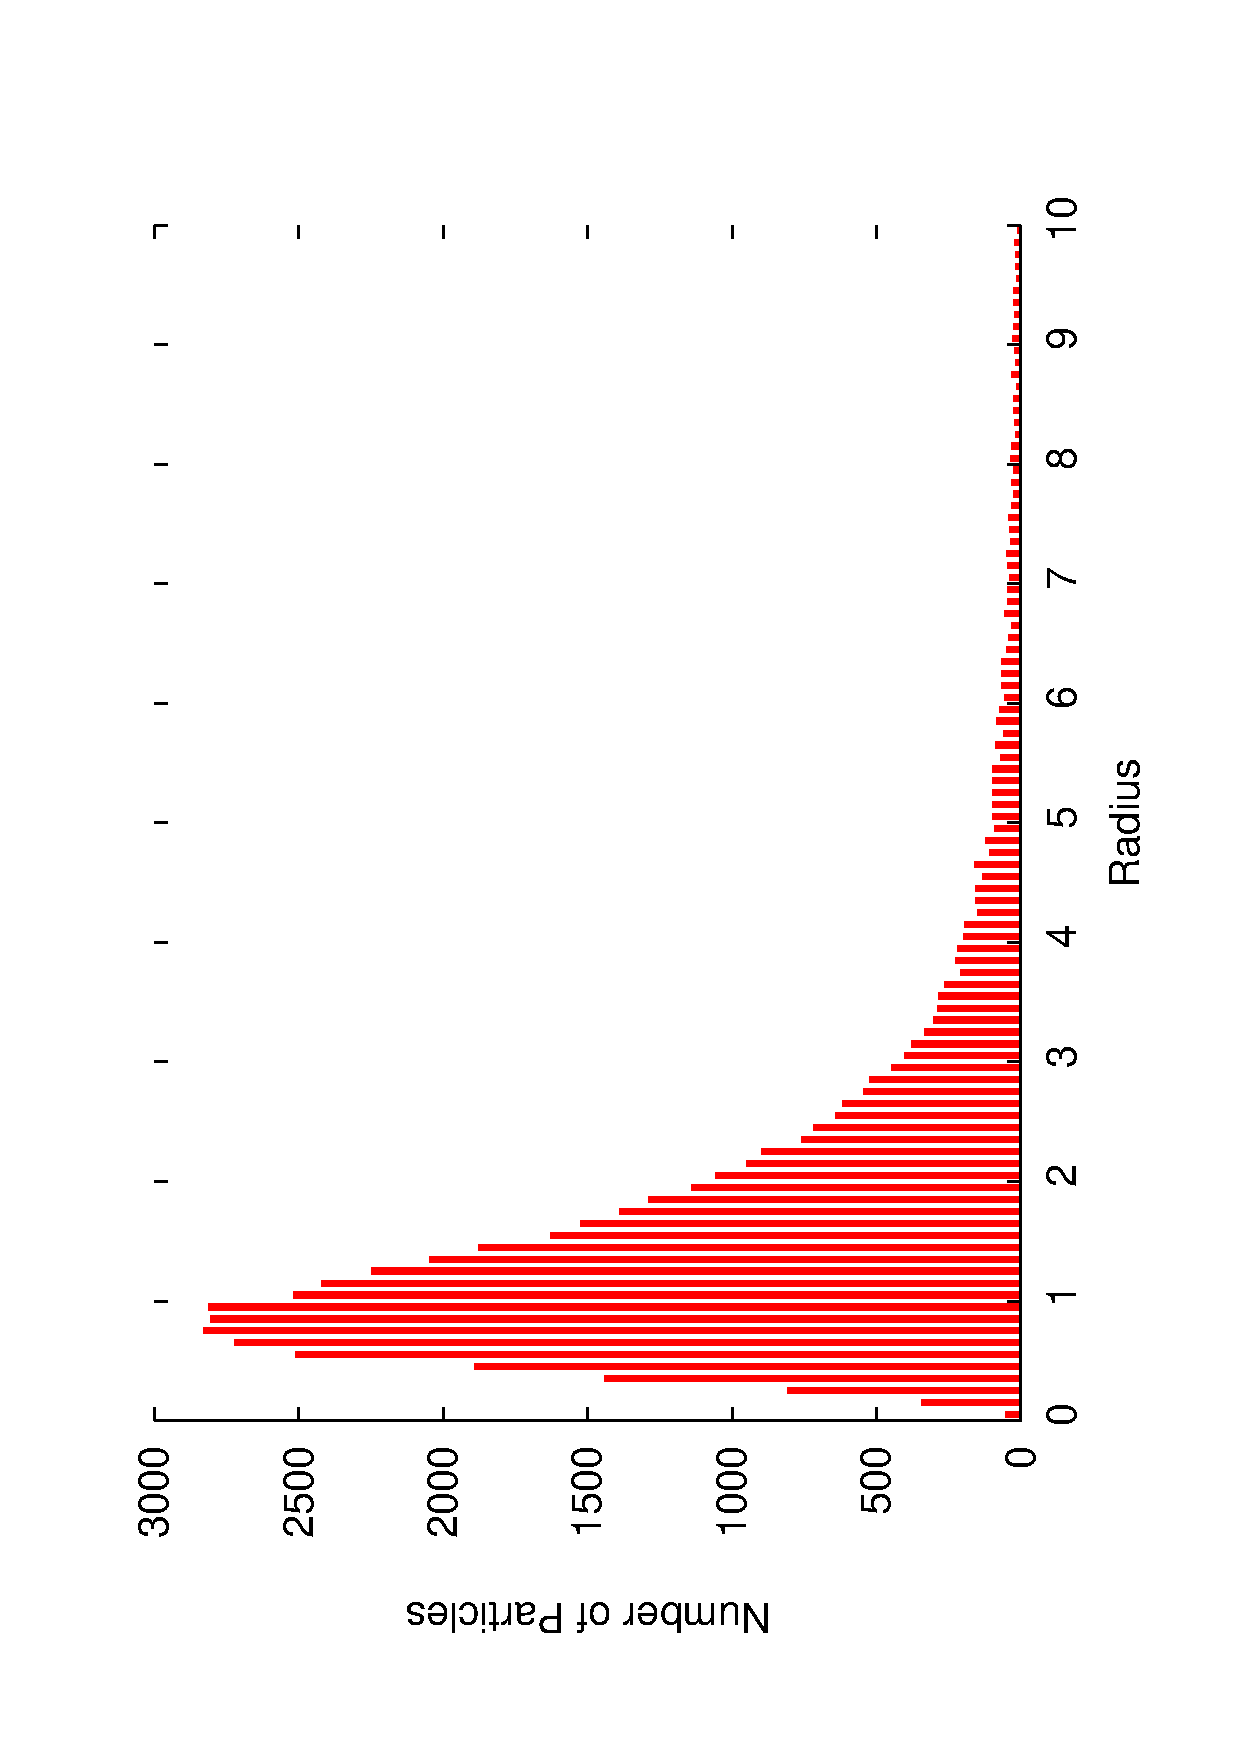
\includegraphics[scale=0.37,angle=-90]{plummerHistogramme}
    \caption{Radius distribution}%
  \end{minipage}%
   \qquad
  \begin{minipage}{0.45\textwidth}%
   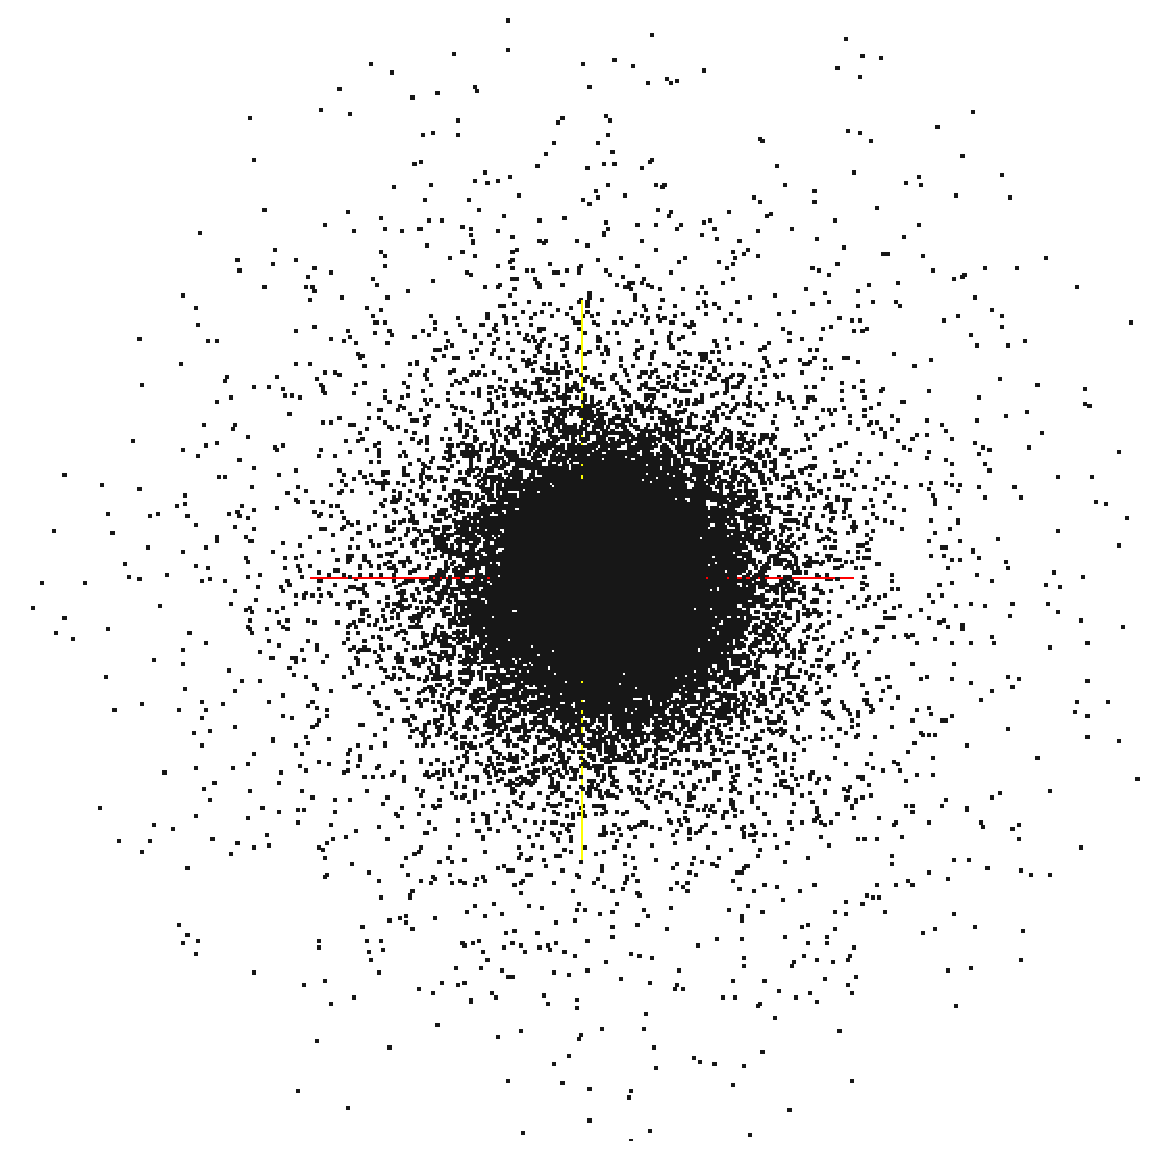
\includegraphics[width=1.0\textwidth]{plummer3D}
    \caption{$50\,000$ point distribution.}%
      \end{minipage}%

\end{figure}

The command to generate such distribution is\\
\texttt{generateDistributions -plummer -radius 10 -N 50000 -fout plummer.bfma  -fvisuout plummer.vtp 
} 



The Plummer 3-dimensional density profile is 
\begin{equation}
\rho_P(r) = \frac{3 M}{4\pi a^3} (1+\frac{r^2}{a^2})^{-\frac{5}{2}}
\end{equation}
where M is the total mass of the cluster and $a$ the Plummer radius. 

The corresponding potential is 
\begin{equation}
\Phi_P(r) = - \frac{G M}{\sqrt{r^2+a^2}}
\end{equation}

In N-body units, $G = M = 1$ and $a = 3\pi/16 \sim 0.589$
\subsection{Diagonal Model}

%, shape end size=.5cm},decoration={shape start size=.5cm, shape end size=.125cm
\tikzset{bigger/.style={decoration={shape start size=.125cm}}}
\tikzset{myblack/.style={draw,fill=black}}

  \begin{tikzpicture}[scale=0.5]
  Lmax = 2; 
  a := 10; 
  \foreach \l in {1,2,3,4,5} {
	\draw (10-20/2^\l,10-10/2^\l) -- (10.0,10-10/2^\l)  ;
	\draw (10-10/2^\l,10-20/2^\l) -- (10-10/2^\l,10.0)  ;
	\draw [myblack] (10-15/2^\l,10-15/2^\l) circle (0.1) ;
    }
    \draw [myblack] (10-5/2^5,10-5/2^5) circle (0.1) ;

  \draw (0,0) rectangle (10,10);
\end{tikzpicture}
%	\node at (10-15/2^\l,10-15/2^\l) [shape=circle,size=6mm,draw=black,fill=black] {} ;


  \begin{tikzpicture}[scale=0.5]
  Lmax = 2; 
  a := 10; 
  \foreach \l in {1,2,3,4,5} {
	\draw (10-20/2^\l,10-10/2^\l) -- (10.0,10-10/2^\l)  ;
	\draw (10-10/2^\l,10-20/2^\l) -- (10-10/2^\l,10.0)  ;
	\draw [myblack] (10-15/2^\l,10-15/2^\l) circle (0.1) ;
    }
    \draw [myblack] (10-5/2^5,10-5/2^5) circle (0.1) ;

  \draw (0,0) rectangle (10,10);
\end{tikzpicture}
\newpage
\begin{thebibliography}{1}
\bibitem{Williamson} J. F. Williamson, “Random selection of points distributed on curved surfaces,” Physics in Medicine and Biology, vol. 32, no. 10, pp. 1311–1319, Oct. 1987.

\bibitem{ChenGlotzer} T. Chen and S. C. Glotzer, “Simulation studies of a phenomenological model for elongated virus capsid formation,” Physical review. E, Statistical, nonlinear, and soft matter physics, vol. 75, pp. 1–25, 2007.

\end{thebibliography}

\newpage
\section{Annexe}
\subsection{Gnuplot script for histogram}
\begin{verbatim}
clear
reset
set key off
set border 3
# Add a vertical dotted line at x=0 to show centre (mean) of distribution.
set yzeroaxis

# Each bar is half the (visual) width of its x-range.
set boxwidth 0.05 absolute
set style fill solid 1.0 noborder

bin_width = 0.1;

bin_number(x) = floor(x/bin_width)

rounded(x) = bin_width * ( bin_number(x) + 0.5 )

set xlabel "Radius"
set ylabel "Number of Particles"

#set terminal postscript enhanced color  'Helvetica' 20
#set output 'plummerHistogramme.eps'

plot 'plummerNewSort.txt' using (rounded($1)):(1) smooth frequency with boxes
\end{verbatim}
\end{document}
